\documentclass[1p]{elsarticle_modified}
%\bibliographystyle{elsarticle-num}

%\usepackage[colorlinks]{hyperref}
%\usepackage{abbrmath_seonhwa} %\Abb, \Ascr, \Acal ,\Abf, \Afrak
\usepackage{amsfonts}
\usepackage{amssymb}
\usepackage{amsmath}
\usepackage{amsthm}
\usepackage{scalefnt}
\usepackage{amsbsy}
\usepackage{kotex}
\usepackage{caption}
\usepackage{subfig}
\usepackage{color}
\usepackage{graphicx}
\usepackage{xcolor} %% white, black, red, green, blue, cyan, magenta, yellow
\usepackage{float}
\usepackage{setspace}
\usepackage{hyperref}

\usepackage{tikz}
\usetikzlibrary{arrows}

\usepackage{multirow}
\usepackage{array} % fixed length table
\usepackage{hhline}

%%%%%%%%%%%%%%%%%%%%%
\makeatletter
\renewcommand*\env@matrix[1][\arraystretch]{%
	\edef\arraystretch{#1}%
	\hskip -\arraycolsep
	\let\@ifnextchar\new@ifnextchar
	\array{*\c@MaxMatrixCols c}}
\makeatother %https://tex.stackexchange.com/questions/14071/how-can-i-increase-the-line-spacing-in-a-matrix
%%%%%%%%%%%%%%%

\usepackage[normalem]{ulem}

\newcommand{\msout}[1]{\ifmmode\text{\sout{\ensuremath{#1}}}\else\sout{#1}\fi}
%SOURCE: \msout is \stkout macro in https://tex.stackexchange.com/questions/20609/strikeout-in-math-mode

\newcommand{\cancel}[1]{
	\ifmmode
	{\color{red}\msout{#1}}
	\else
	{\color{red}\sout{#1}}
	\fi
}

\newcommand{\add}[1]{
	{\color{blue}\uwave{#1}}
}

\newcommand{\replace}[2]{
	\ifmmode
	{\color{red}\msout{#1}}{\color{blue}\uwave{#2}}
	\else
	{\color{red}\sout{#1}}{\color{blue}\uwave{#2}}
	\fi
}

\newcommand{\Sol}{\mathcal{S}} %segment
\newcommand{\D}{D} %diagram
\newcommand{\A}{\mathcal{A}} %arc


%%%%%%%%%%%%%%%%%%%%%%%%%%%%%5 test

\def\sl{\operatorname{\textup{SL}}(2,\Cbb)}
\def\psl{\operatorname{\textup{PSL}}(2,\Cbb)}
\def\quan{\mkern 1mu \triangleright \mkern 1mu}

\theoremstyle{definition}
\newtheorem{thm}{Theorem}[section]
\newtheorem{prop}[thm]{Proposition}
\newtheorem{lem}[thm]{Lemma}
\newtheorem{ques}[thm]{Question}
\newtheorem{cor}[thm]{Corollary}
\newtheorem{defn}[thm]{Definition}
\newtheorem{exam}[thm]{Example}
\newtheorem{rmk}[thm]{Remark}
\newtheorem{alg}[thm]{Algorithm}

\newcommand{\I}{\sqrt{-1}}
\begin{document}

%\begin{frontmatter}
%
%\title{Boundary parabolic representations of knots up to 8 crossings}
%
%%% Group authors per affiliation:
%\author{Yunhi Cho} 
%\address{Department of Mathematics, University of Seoul, Seoul, Korea}
%\ead{yhcho@uos.ac.kr}
%
%
%\author{Seonhwa Kim} %\fnref{s_kim}}
%\address{Center for Geometry and Physics, Institute for Basic Science, Pohang, 37673, Korea}
%\ead{ryeona17@ibs.re.kr}
%
%\author{Hyuk Kim}
%\address{Department of Mathematical Sciences, Seoul National University, Seoul 08826, Korea}
%\ead{hyukkim@snu.ac.kr}
%
%\author{Seokbeom Yoon}
%\address{Department of Mathematical Sciences, Seoul National University, Seoul, 08826,  Korea}
%\ead{sbyoon15@snu.ac.kr}
%
%\begin{abstract}
%We find all boundary parabolic representation of knots up to 8 crossings.
%
%\end{abstract}
%\begin{keyword}
%    \MSC[2010] 57M25 
%\end{keyword}
%
%\end{frontmatter}

%\linenumbers
%\tableofcontents
%
\newcommand\colored[1]{\textcolor{white}{\rule[-0.35ex]{0.8em}{1.4ex}}\kern-0.8em\color{red} #1}%
%\newcommand\colored[1]{\textcolor{white}{ #1}\kern-2.17ex	\textcolor{white}{ #1}\kern-1.81ex	\textcolor{white}{ #1}\kern-2.15ex\color{red}#1	}

{\Large $\underline{12n_{0782}~(K12n_{0782})}$}

\setlength{\tabcolsep}{10pt}
\renewcommand{\arraystretch}{1.6}
\vspace{1cm}\begin{tabular}{m{100pt}>{\centering\arraybackslash}m{274pt}}
\multirow{5}{120pt}{
	\centering
	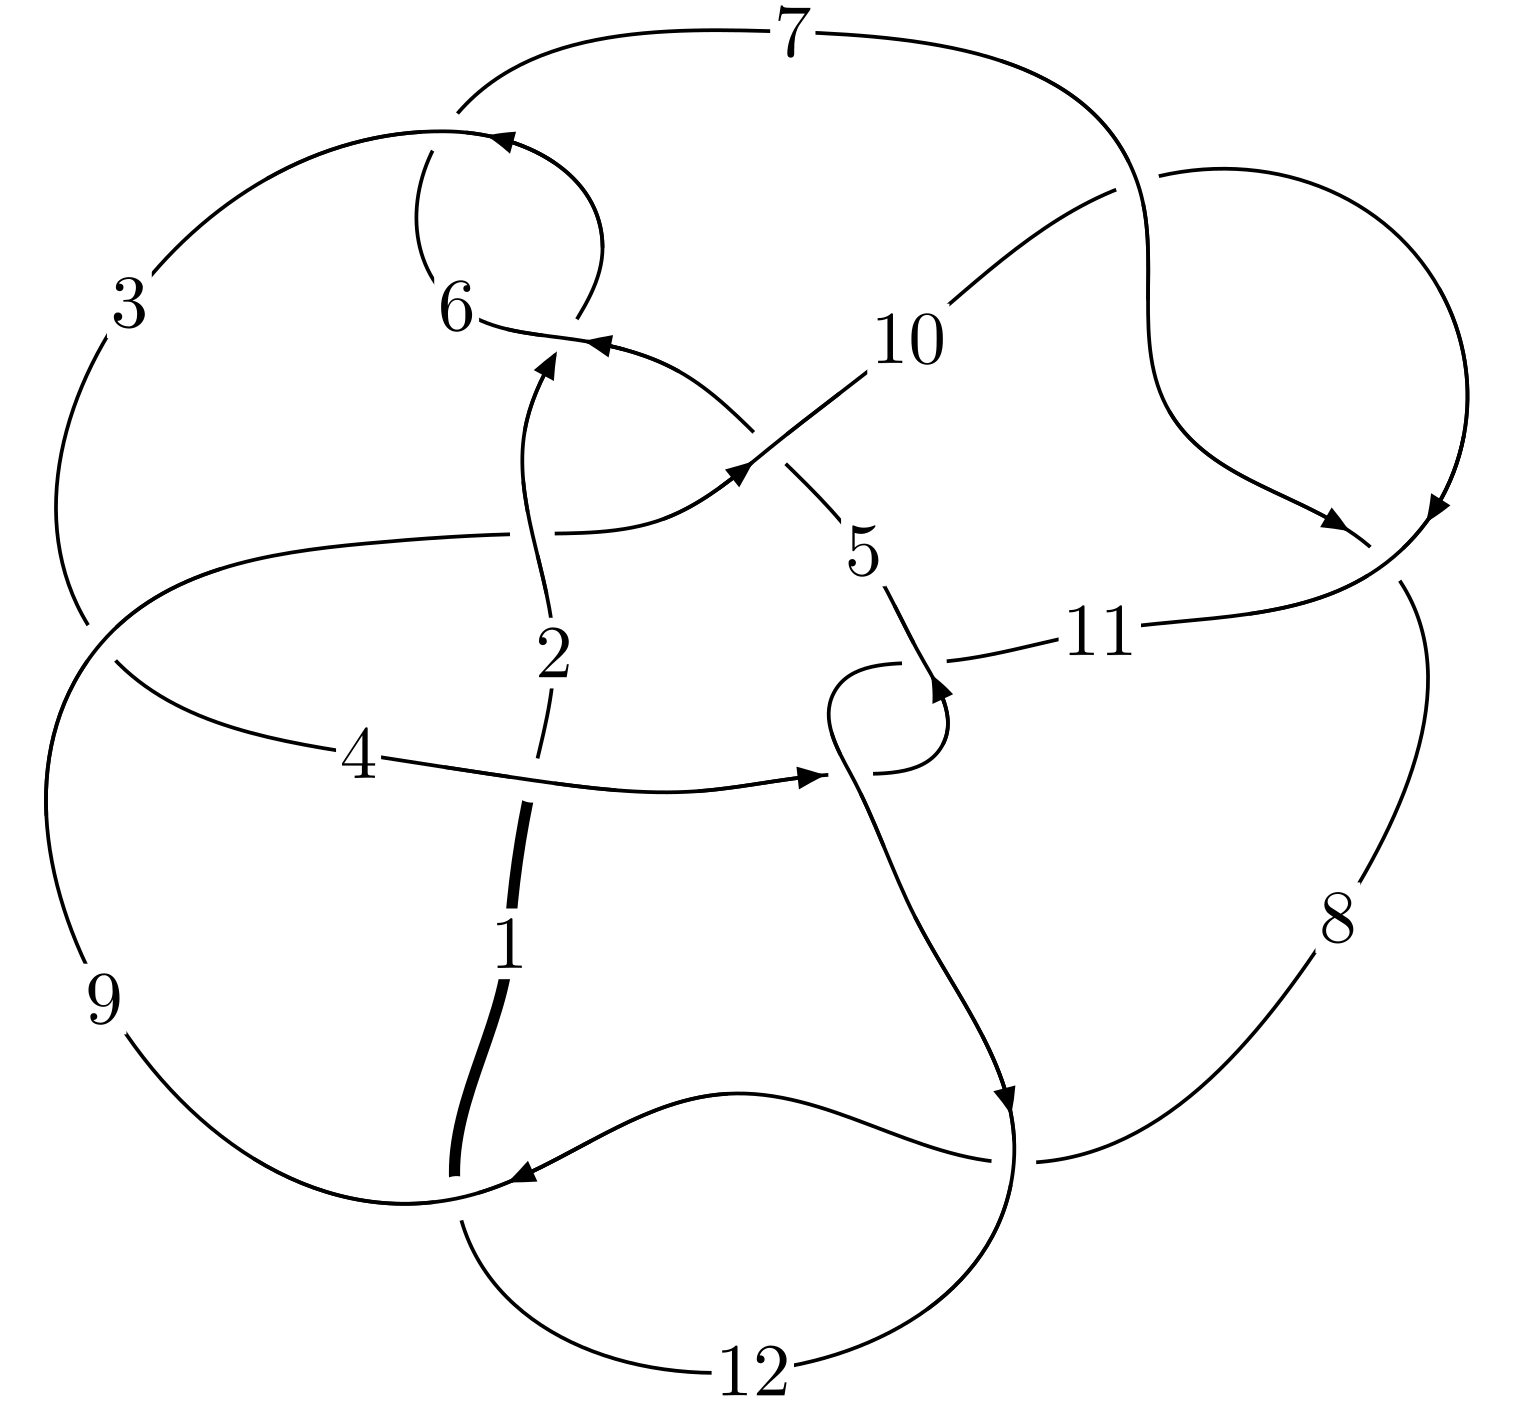
\includegraphics[width=112pt]{../../../GIT/diagram.site/Diagrams/png/2871_12n_0782.png}\\
\ \ \ A knot diagram\footnotemark}&
\allowdisplaybreaks
\textbf{Linearized knot diagam} \\
\cline{2-2}
 &
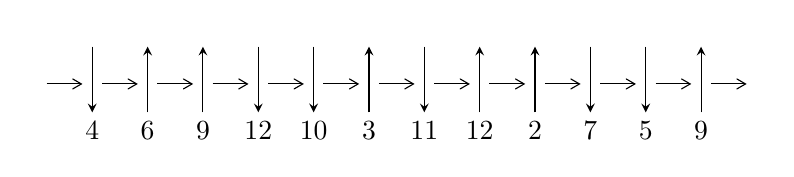
\begin{tikzpicture}[x=20pt, y=17pt]
	% nodes
	\node (C0) at (0, 0) {};
	\node (C1) at (1, 0) {};
	\node (C1U) at (1, +1) {};
	\node (C1D) at (1, -1) {4};

	\node (C2) at (2, 0) {};
	\node (C2U) at (2, +1) {};
	\node (C2D) at (2, -1) {6};

	\node (C3) at (3, 0) {};
	\node (C3U) at (3, +1) {};
	\node (C3D) at (3, -1) {9};

	\node (C4) at (4, 0) {};
	\node (C4U) at (4, +1) {};
	\node (C4D) at (4, -1) {12};

	\node (C5) at (5, 0) {};
	\node (C5U) at (5, +1) {};
	\node (C5D) at (5, -1) {10};

	\node (C6) at (6, 0) {};
	\node (C6U) at (6, +1) {};
	\node (C6D) at (6, -1) {3};

	\node (C7) at (7, 0) {};
	\node (C7U) at (7, +1) {};
	\node (C7D) at (7, -1) {11};

	\node (C8) at (8, 0) {};
	\node (C8U) at (8, +1) {};
	\node (C8D) at (8, -1) {12};

	\node (C9) at (9, 0) {};
	\node (C9U) at (9, +1) {};
	\node (C9D) at (9, -1) {2};

	\node (C10) at (10, 0) {};
	\node (C10U) at (10, +1) {};
	\node (C10D) at (10, -1) {7};

	\node (C11) at (11, 0) {};
	\node (C11U) at (11, +1) {};
	\node (C11D) at (11, -1) {5};

	\node (C12) at (12, 0) {};
	\node (C12U) at (12, +1) {};
	\node (C12D) at (12, -1) {9};
	\node (C13) at (13, 0) {};

	% arrows
	\draw[->,>={angle 60}]
	(C0) edge (C1) (C1) edge (C2) (C2) edge (C3) (C3) edge (C4) (C4) edge (C5) (C5) edge (C6) (C6) edge (C7) (C7) edge (C8) (C8) edge (C9) (C9) edge (C10) (C10) edge (C11) (C11) edge (C12) (C12) edge (C13) ;	\draw[->,>=stealth]
	(C1U) edge (C1D) (C2D) edge (C2U) (C3D) edge (C3U) (C4U) edge (C4D) (C5U) edge (C5D) (C6D) edge (C6U) (C7U) edge (C7D) (C8D) edge (C8U) (C9D) edge (C9U) (C10U) edge (C10D) (C11U) edge (C11D) (C12D) edge (C12U) ;
	\end{tikzpicture} \\
\hhline{~~} \\& 
\textbf{Solving Sequence} \\ \cline{2-2} 
 &
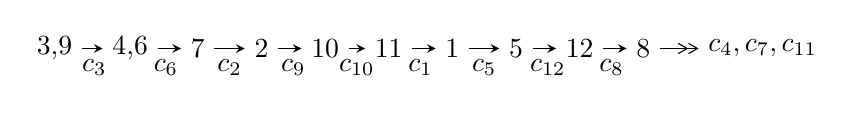
\begin{tikzpicture}[x=23pt, y=7pt]
	% node
	\node (A0) at (-1/8, 0) {3,9};
	\node (A1) at (17/16, 0) {4,6};
	\node (A2) at (17/8, 0) {7};
	\node (A3) at (25/8, 0) {2};
	\node (A4) at (33/8, 0) {10};
	\node (A5) at (41/8, 0) {11};
	\node (A6) at (49/8, 0) {1};
	\node (A7) at (57/8, 0) {5};
	\node (A8) at (65/8, 0) {12};
	\node (A9) at (73/8, 0) {8};
	\node (C1) at (1/2, -1) {$c_{3}$};
	\node (C2) at (13/8, -1) {$c_{6}$};
	\node (C3) at (21/8, -1) {$c_{2}$};
	\node (C4) at (29/8, -1) {$c_{9}$};
	\node (C5) at (37/8, -1) {$c_{10}$};
	\node (C6) at (45/8, -1) {$c_{1}$};
	\node (C7) at (53/8, -1) {$c_{5}$};
	\node (C8) at (61/8, -1) {$c_{12}$};
	\node (C9) at (69/8, -1) {$c_{8}$};
	\node (A10) at (11, 0) {$c_{4},c_{7},c_{11}$};

	% edge
	\draw[->,>=stealth]	
	(A0) edge (A1) (A1) edge (A2) (A2) edge (A3) (A3) edge (A4) (A4) edge (A5) (A5) edge (A6) (A6) edge (A7) (A7) edge (A8) (A8) edge (A9) ;
	\draw[->>,>={angle 60}]	
	(A9) edge (A10);
\end{tikzpicture} \\ 

\end{tabular} \\

\footnotetext{
The image of knot diagram is generated by the software ``\textbf{Draw programme}" developed by Andrew Bartholomew(\url{http://www.layer8.co.uk/maths/draw/index.htm\#Running-draw}), where we modified some parts for our purpose(\url{https://github.com/CATsTAILs/LinksPainter}).
}\phantom \\ \newline 
\centering \textbf{Ideals for irreducible components\footnotemark of $X_{\text{par}}$} 
 
\begin{align*}
I^u_{1}&=\langle 
5.27881\times10^{88} u^{57}-4.69361\times10^{90} u^{56}+\cdots+1.36590\times10^{92} b-5.88184\times10^{92},\\
\phantom{I^u_{1}}&\phantom{= \langle  }-2.96745\times10^{93} u^{57}-2.47917\times10^{93} u^{56}+\cdots+8.04515\times10^{94} a+3.43955\times10^{95},\\
\phantom{I^u_{1}}&\phantom{= \langle  }u^{58}+u^{57}+\cdots-223 u+38\rangle \\
I^u_{2}&=\langle 
475169 u^{17}+381386 u^{16}+\cdots+522553 b+471664,\\
\phantom{I^u_{2}}&\phantom{= \langle  }-688088 u^{17}-1519820 u^{16}+\cdots+2612765 a-1890667,\;u^{18}+15 u^{16}+\cdots-6 u+5\rangle \\
\\
\end{align*}
\raggedright * 2 irreducible components of $\dim_{\mathbb{C}}=0$, with total 76 representations.\\
\footnotetext{All coefficients of polynomials are rational numbers. But the coefficients are sometimes approximated in decimal forms when there is not enough margin.}
\newpage
\renewcommand{\arraystretch}{1}
\centering \section*{I. $I^u_{1}= \langle 5.28\times10^{88} u^{57}-4.69\times10^{90} u^{56}+\cdots+1.37\times10^{92} b-5.88\times10^{92},\;-2.97\times10^{93} u^{57}-2.48\times10^{93} u^{56}+\cdots+8.05\times10^{94} a+3.44\times10^{95},\;u^{58}+u^{57}+\cdots-223 u+38 \rangle$}
\flushleft \textbf{(i) Arc colorings}\\
\begin{tabular}{m{7pt} m{180pt} m{7pt} m{180pt} }
\flushright $a_{3}=$&$\begin{pmatrix}1\\0\end{pmatrix}$ \\
\flushright $a_{9}=$&$\begin{pmatrix}0\\u\end{pmatrix}$ \\
\flushright $a_{4}=$&$\begin{pmatrix}1\\- u^2\end{pmatrix}$ \\
\flushright $a_{6}=$&$\begin{pmatrix}0.0368850 u^{57}+0.0308157 u^{56}+\cdots+41.2134 u-4.27531\\-0.000386471 u^{57}+0.0343628 u^{56}+\cdots-23.7709 u+4.30620\end{pmatrix}$ \\
\flushright $a_{7}=$&$\begin{pmatrix}0.0364985 u^{57}+0.0651785 u^{56}+\cdots+17.4426 u+0.0308943\\-0.000386471 u^{57}+0.0343628 u^{56}+\cdots-23.7709 u+4.30620\end{pmatrix}$ \\
\flushright $a_{2}=$&$\begin{pmatrix}0.0405848 u^{57}+0.0585166 u^{56}+\cdots+63.4140 u-5.65068\\-0.0519284 u^{57}-0.0695194 u^{56}+\cdots-12.5917 u+0.686208\end{pmatrix}$ \\
\flushright $a_{10}=$&$\begin{pmatrix}-0.106783 u^{57}-0.120253 u^{56}+\cdots-87.1353 u+3.59553\\0.0335600 u^{57}+0.0556513 u^{56}+\cdots+0.799424 u+0.951777\end{pmatrix}$ \\
\flushright $a_{11}=$&$\begin{pmatrix}0.00494700 u^{57}+0.0479532 u^{56}+\cdots-57.8669 u+5.20437\\0.0678161 u^{57}+0.0966838 u^{56}+\cdots-15.7287 u+4.42152\end{pmatrix}$ \\
\flushright $a_{1}=$&$\begin{pmatrix}-0.00916084 u^{57}-0.0269986 u^{56}+\cdots+53.2788 u-5.64588\\-0.0924440 u^{57}-0.175276 u^{56}+\cdots-6.50545 u-0.673036\end{pmatrix}$ \\
\flushright $a_{5}=$&$\begin{pmatrix}0.00126585 u^{57}+0.0187770 u^{56}+\cdots-50.5853 u+14.2462\\0.0175336 u^{57}+0.00565385 u^{56}+\cdots-1.20624 u+0.716555\end{pmatrix}$ \\
\flushright $a_{12}=$&$\begin{pmatrix}-0.00916084 u^{57}-0.0269986 u^{56}+\cdots+53.2788 u-5.64588\\-0.0497456 u^{57}-0.0855152 u^{56}+\cdots-10.1352 u+0.00479944\end{pmatrix}$ \\
\flushright $a_{8}=$&$\begin{pmatrix}0.0258619 u^{57}+0.106305 u^{56}+\cdots+55.7975 u-1.95424\\-0.0553761 u^{57}+0.0473162 u^{56}+\cdots-29.4845 u+3.10494\end{pmatrix}$\\&\end{tabular}
\flushleft \textbf{(ii) Obstruction class $= -1$}\\~\\
\flushleft \textbf{(iii) Cusp Shapes $= -0.0872911 u^{57}-0.355385 u^{56}+\cdots+59.4278 u-12.0616$}\\~\\
\newpage\renewcommand{\arraystretch}{1}
\flushleft \textbf{(iv) u-Polynomials at the component}\newline \\
\begin{tabular}{m{50pt}|m{274pt}}
Crossings & \hspace{64pt}u-Polynomials at each crossing \\
\hline $$\begin{aligned}c_{1}\end{aligned}$$&$\begin{aligned}
&u^{58}-8 u^{57}+\cdots-59912 u+5747
\end{aligned}$\\
\hline $$\begin{aligned}c_{2},c_{6}\end{aligned}$$&$\begin{aligned}
&u^{58}-13 u^{56}+\cdots-638 u+247
\end{aligned}$\\
\hline $$\begin{aligned}c_{3}\end{aligned}$$&$\begin{aligned}
&u^{58}- u^{57}+\cdots+223 u+38
\end{aligned}$\\
\hline $$\begin{aligned}c_{4},c_{11}\end{aligned}$$&$\begin{aligned}
&u^{58}+2 u^{57}+\cdots-4 u+47
\end{aligned}$\\
\hline $$\begin{aligned}c_{5}\end{aligned}$$&$\begin{aligned}
&u^{58}- u^{57}+\cdots-155 u+118
\end{aligned}$\\
\hline $$\begin{aligned}c_{7},c_{10}\end{aligned}$$&$\begin{aligned}
&u^{58}+3 u^{57}+\cdots+410 u+25
\end{aligned}$\\
\hline $$\begin{aligned}c_{8},c_{12}\end{aligned}$$&$\begin{aligned}
&u^{58}+45 u^{56}+\cdots+1851 u+269
\end{aligned}$\\
\hline $$\begin{aligned}c_{9}\end{aligned}$$&$\begin{aligned}
&u^{58}- u^{57}+\cdots-22 u+97
\end{aligned}$\\
\hline
\end{tabular}\\~\\
\newpage\renewcommand{\arraystretch}{1}
\flushleft \textbf{(v) Riley Polynomials at the component}\newline \\
\begin{tabular}{m{50pt}|m{274pt}}
Crossings & \hspace{64pt}Riley Polynomials at each crossing \\
\hline $$\begin{aligned}c_{1}\end{aligned}$$&$\begin{aligned}
&y^{58}-84 y^{57}+\cdots+622723954 y+33028009
\end{aligned}$\\
\hline $$\begin{aligned}c_{2},c_{6}\end{aligned}$$&$\begin{aligned}
&y^{58}-26 y^{57}+\cdots-629838 y+61009
\end{aligned}$\\
\hline $$\begin{aligned}c_{3}\end{aligned}$$&$\begin{aligned}
&y^{58}+75 y^{57}+\cdots+81523 y+1444
\end{aligned}$\\
\hline $$\begin{aligned}c_{4},c_{11}\end{aligned}$$&$\begin{aligned}
&y^{58}+2 y^{57}+\cdots+4120 y+2209
\end{aligned}$\\
\hline $$\begin{aligned}c_{5}\end{aligned}$$&$\begin{aligned}
&y^{58}+31 y^{57}+\cdots+80523 y+13924
\end{aligned}$\\
\hline $$\begin{aligned}c_{7},c_{10}\end{aligned}$$&$\begin{aligned}
&y^{58}-53 y^{57}+\cdots-18700 y+625
\end{aligned}$\\
\hline $$\begin{aligned}c_{8},c_{12}\end{aligned}$$&$\begin{aligned}
&y^{58}+90 y^{57}+\cdots+3009893 y+72361
\end{aligned}$\\
\hline $$\begin{aligned}c_{9}\end{aligned}$$&$\begin{aligned}
&y^{58}-23 y^{57}+\cdots-9020 y+9409
\end{aligned}$\\
\hline
\end{tabular}\\~\\
\newpage\flushleft \textbf{(vi) Complex Volumes and Cusp Shapes}
$$\begin{array}{c|c|c}  
\text{Solutions to }I^u_{1}& \I (\text{vol} + \sqrt{-1}CS) & \text{Cusp shape}\\
 \hline 
\begin{aligned}
u &= \phantom{-}0.853751 + 0.464332 I \\
a &= -0.0493088 - 0.0773017 I \\
b &= \phantom{-}0.203439 - 1.110150 I\end{aligned}
 & -2.63383 + 3.87803 I & \phantom{-0.000000 } 0. - 7.10067 I \\ \hline\begin{aligned}
u &= \phantom{-}0.853751 - 0.464332 I \\
a &= -0.0493088 + 0.0773017 I \\
b &= \phantom{-}0.203439 + 1.110150 I\end{aligned}
 & -2.63383 - 3.87803 I & \phantom{-0.000000 -}0. + 7.10067 I \\ \hline\begin{aligned}
u &= -1.062870 + 0.155680 I \\
a &= \phantom{-}1.383060 + 0.177575 I \\
b &= -1.287020 + 0.256764 I\end{aligned}
 & \phantom{-}3.11643 - 0.54489 I & \phantom{-0.000000 } 0 \\ \hline\begin{aligned}
u &= -1.062870 - 0.155680 I \\
a &= \phantom{-}1.383060 - 0.177575 I \\
b &= -1.287020 - 0.256764 I\end{aligned}
 & \phantom{-}3.11643 + 0.54489 I & \phantom{-0.000000 } 0 \\ \hline\begin{aligned}
u &= -0.112581 + 0.912921 I \\
a &= \phantom{-}0.15835 + 1.82362 I \\
b &= -0.965630 + 0.677508 I\end{aligned}
 & \phantom{-}6.95013 - 2.72728 I & \phantom{-}5.05992 + 2.76752 I \\ \hline\begin{aligned}
u &= -0.112581 - 0.912921 I \\
a &= \phantom{-}0.15835 - 1.82362 I \\
b &= -0.965630 - 0.677508 I\end{aligned}
 & \phantom{-}6.95013 + 2.72728 I & \phantom{-}5.05992 - 2.76752 I \\ \hline\begin{aligned}
u &= -0.084433 + 0.832538 I \\
a &= \phantom{-}0.0357940 + 0.0140818 I \\
b &= \phantom{-}1.140920 - 0.525982 I\end{aligned}
 & -0.82014 - 4.75740 I & -0.14886 + 5.79153 I \\ \hline\begin{aligned}
u &= -0.084433 - 0.832538 I \\
a &= \phantom{-}0.0357940 - 0.0140818 I \\
b &= \phantom{-}1.140920 + 0.525982 I\end{aligned}
 & -0.82014 + 4.75740 I & -0.14886 - 5.79153 I \\ \hline\begin{aligned}
u &= \phantom{-}0.782245 + 0.038291 I \\
a &= -1.99589 - 0.35305 I \\
b &= \phantom{-}1.222820 + 0.263072 I\end{aligned}
 & \phantom{-}4.17334 + 3.33228 I & \phantom{-}6.92799 - 6.82937 I \\ \hline\begin{aligned}
u &= \phantom{-}0.782245 - 0.038291 I \\
a &= -1.99589 + 0.35305 I \\
b &= \phantom{-}1.222820 - 0.263072 I\end{aligned}
 & \phantom{-}4.17334 - 3.33228 I & \phantom{-}6.92799 + 6.82937 I\\
 \hline 
 \end{array}$$\newpage$$\begin{array}{c|c|c}  
\text{Solutions to }I^u_{1}& \I (\text{vol} + \sqrt{-1}CS) & \text{Cusp shape}\\
 \hline 
\begin{aligned}
u &= \phantom{-}0.099784 + 1.239980 I \\
a &= \phantom{-}0.46372 - 1.67392 I \\
b &= -0.933454 - 0.370814 I\end{aligned}
 & \phantom{-}1.66999 + 1.54564 I & \phantom{-0.000000 } 0 \\ \hline\begin{aligned}
u &= \phantom{-}0.099784 - 1.239980 I \\
a &= \phantom{-}0.46372 + 1.67392 I \\
b &= -0.933454 + 0.370814 I\end{aligned}
 & \phantom{-}1.66999 - 1.54564 I & \phantom{-0.000000 } 0 \\ \hline\begin{aligned}
u &= -0.014033 + 1.261280 I \\
a &= \phantom{-}0.753664 - 0.681102 I \\
b &= -0.889945 - 0.068116 I\end{aligned}
 & \phantom{-}0.047703 + 0.198149 I & \phantom{-0.000000 } 0 \\ \hline\begin{aligned}
u &= -0.014033 - 1.261280 I \\
a &= \phantom{-}0.753664 + 0.681102 I \\
b &= -0.889945 + 0.068116 I\end{aligned}
 & \phantom{-}0.047703 - 0.198149 I & \phantom{-0.000000 } 0 \\ \hline\begin{aligned}
u &= -0.450292 + 1.192360 I \\
a &= -0.624837 - 0.475798 I \\
b &= \phantom{-}1.338790 - 0.213313 I\end{aligned}
 & -0.33330 - 4.75057 I & \phantom{-0.000000 } 0 \\ \hline\begin{aligned}
u &= -0.450292 - 1.192360 I \\
a &= -0.624837 + 0.475798 I \\
b &= \phantom{-}1.338790 + 0.213313 I\end{aligned}
 & -0.33330 + 4.75057 I & \phantom{-0.000000 } 0 \\ \hline\begin{aligned}
u &= \phantom{-}0.003350 + 1.288710 I \\
a &= -0.209714 - 0.410378 I \\
b &= \phantom{-}0.136782 - 1.254630 I\end{aligned}
 & -4.85427 - 1.06680 I & \phantom{-0.000000 } 0 \\ \hline\begin{aligned}
u &= \phantom{-}0.003350 - 1.288710 I \\
a &= -0.209714 + 0.410378 I \\
b &= \phantom{-}0.136782 + 1.254630 I\end{aligned}
 & -4.85427 + 1.06680 I & \phantom{-0.000000 } 0 \\ \hline\begin{aligned}
u &= \phantom{-}0.314738 + 1.298090 I \\
a &= \phantom{-}1.025510 - 0.858022 I \\
b &= -1.39942 - 0.56356 I\end{aligned}
 & \phantom{-}0.00633 + 7.27891 I & \phantom{-0.000000 } 0 \\ \hline\begin{aligned}
u &= \phantom{-}0.314738 - 1.298090 I \\
a &= \phantom{-}1.025510 + 0.858022 I \\
b &= -1.39942 + 0.56356 I\end{aligned}
 & \phantom{-}0.00633 - 7.27891 I & \phantom{-0.000000 } 0\\
 \hline 
 \end{array}$$\newpage$$\begin{array}{c|c|c}  
\text{Solutions to }I^u_{1}& \I (\text{vol} + \sqrt{-1}CS) & \text{Cusp shape}\\
 \hline 
\begin{aligned}
u &= -1.123890 + 0.727662 I \\
a &= -1.289100 - 0.536945 I \\
b &= \phantom{-}1.288900 - 0.578954 I\end{aligned}
 & \phantom{-}0.86445 - 9.82160 I & \phantom{-0.000000 } 0 \\ \hline\begin{aligned}
u &= -1.123890 - 0.727662 I \\
a &= -1.289100 + 0.536945 I \\
b &= \phantom{-}1.288900 + 0.578954 I\end{aligned}
 & \phantom{-}0.86445 + 9.82160 I & \phantom{-0.000000 } 0 \\ \hline\begin{aligned}
u &= \phantom{-}0.460864 + 0.418666 I \\
a &= \phantom{-}0.57224 - 1.90811 I \\
b &= \phantom{-}0.385032 - 0.536811 I\end{aligned}
 & -3.08131 + 0.52947 I & -3.73900 + 2.26505 I \\ \hline\begin{aligned}
u &= \phantom{-}0.460864 - 0.418666 I \\
a &= \phantom{-}0.57224 + 1.90811 I \\
b &= \phantom{-}0.385032 + 0.536811 I\end{aligned}
 & -3.08131 - 0.52947 I & -3.73900 - 2.26505 I \\ \hline\begin{aligned}
u &= -0.124818 + 0.519430 I \\
a &= -1.71837 - 1.68133 I \\
b &= \phantom{-}0.919845 + 0.470366 I\end{aligned}
 & \phantom{-}8.22063 + 1.95332 I & -4.24227 - 5.07597 I \\ \hline\begin{aligned}
u &= -0.124818 - 0.519430 I \\
a &= -1.71837 + 1.68133 I \\
b &= \phantom{-}0.919845 - 0.470366 I\end{aligned}
 & \phantom{-}8.22063 - 1.95332 I & -4.24227 + 5.07597 I \\ \hline\begin{aligned}
u &= \phantom{-}0.22485 + 1.46017 I \\
a &= \phantom{-}0.043124 - 0.507703 I \\
b &= \phantom{-}0.579349 - 0.997182 I\end{aligned}
 & -5.11981 - 0.34192 I & \phantom{-0.000000 } 0 \\ \hline\begin{aligned}
u &= \phantom{-}0.22485 - 1.46017 I \\
a &= \phantom{-}0.043124 + 0.507703 I \\
b &= \phantom{-}0.579349 + 0.997182 I\end{aligned}
 & -5.11981 + 0.34192 I & \phantom{-0.000000 } 0 \\ \hline\begin{aligned}
u &= \phantom{-}0.164082 + 0.484192 I \\
a &= \phantom{-}1.39498 - 2.02846 I \\
b &= -1.157090 - 0.710262 I\end{aligned}
 & \phantom{-}0.25031 + 5.18394 I & -0.05460 - 3.88348 I \\ \hline\begin{aligned}
u &= \phantom{-}0.164082 - 0.484192 I \\
a &= \phantom{-}1.39498 + 2.02846 I \\
b &= -1.157090 + 0.710262 I\end{aligned}
 & \phantom{-}0.25031 - 5.18394 I & -0.05460 + 3.88348 I\\
 \hline 
 \end{array}$$\newpage$$\begin{array}{c|c|c}  
\text{Solutions to }I^u_{1}& \I (\text{vol} + \sqrt{-1}CS) & \text{Cusp shape}\\
 \hline 
\begin{aligned}
u &= \phantom{-}0.10703 + 1.51586 I \\
a &= \phantom{-}1.05246 + 1.33886 I \\
b &= -0.837740 + 0.446217 I\end{aligned}
 & -9.50824 + 2.34060 I & \phantom{-0.000000 } 0 \\ \hline\begin{aligned}
u &= \phantom{-}0.10703 - 1.51586 I \\
a &= \phantom{-}1.05246 - 1.33886 I \\
b &= -0.837740 - 0.446217 I\end{aligned}
 & -9.50824 - 2.34060 I & \phantom{-0.000000 } 0 \\ \hline\begin{aligned}
u &= -0.03559 + 1.53038 I \\
a &= \phantom{-}0.256243 + 0.650105 I \\
b &= \phantom{-}0.747820 + 1.090540 I\end{aligned}
 & -8.19348 + 0.77858 I & \phantom{-0.000000 } 0 \\ \hline\begin{aligned}
u &= -0.03559 - 1.53038 I \\
a &= \phantom{-}0.256243 - 0.650105 I \\
b &= \phantom{-}0.747820 - 1.090540 I\end{aligned}
 & -8.19348 - 0.77858 I & \phantom{-0.000000 } 0 \\ \hline\begin{aligned}
u &= \phantom{-}0.06553 + 1.55280 I \\
a &= -0.549374 + 1.215700 I \\
b &= \phantom{-}1.141090 + 0.801942 I\end{aligned}
 & -6.78133 + 6.11938 I & \phantom{-0.000000 } 0 \\ \hline\begin{aligned}
u &= \phantom{-}0.06553 - 1.55280 I \\
a &= -0.549374 - 1.215700 I \\
b &= \phantom{-}1.141090 - 0.801942 I\end{aligned}
 & -6.78133 - 6.11938 I & \phantom{-0.000000 } 0 \\ \hline\begin{aligned}
u &= -0.190141 + 0.387639 I \\
a &= \phantom{-}0.446972 - 0.550746 I \\
b &= -0.192799 + 0.357060 I\end{aligned}
 & \phantom{-}0.080144 - 0.948408 I & \phantom{-}1.62310 + 7.11083 I \\ \hline\begin{aligned}
u &= -0.190141 - 0.387639 I \\
a &= \phantom{-}0.446972 + 0.550746 I \\
b &= -0.192799 - 0.357060 I\end{aligned}
 & \phantom{-}0.080144 + 0.948408 I & \phantom{-}1.62310 - 7.11083 I \\ \hline\begin{aligned}
u &= \phantom{-}0.32626 + 1.55223 I \\
a &= -0.241997 + 0.425422 I \\
b &= -0.520923 + 1.219600 I\end{aligned}
 & -9.24266 + 8.26916 I & \phantom{-0.000000 } 0 \\ \hline\begin{aligned}
u &= \phantom{-}0.32626 - 1.55223 I \\
a &= -0.241997 - 0.425422 I \\
b &= -0.520923 - 1.219600 I\end{aligned}
 & -9.24266 - 8.26916 I & \phantom{-0.000000 } 0\\
 \hline 
 \end{array}$$\newpage$$\begin{array}{c|c|c}  
\text{Solutions to }I^u_{1}& \I (\text{vol} + \sqrt{-1}CS) & \text{Cusp shape}\\
 \hline 
\begin{aligned}
u &= -0.26330 + 1.59853 I \\
a &= -0.745743 - 1.025400 I \\
b &= \phantom{-}1.115300 - 0.653239 I\end{aligned}
 & -3.26110 - 5.59088 I & \phantom{-0.000000 } 0 \\ \hline\begin{aligned}
u &= -0.26330 - 1.59853 I \\
a &= -0.745743 + 1.025400 I \\
b &= \phantom{-}1.115300 + 0.653239 I\end{aligned}
 & -3.26110 + 5.59088 I & \phantom{-0.000000 } 0 \\ \hline\begin{aligned}
u &= -0.08919 + 1.63634 I \\
a &= -0.271146 + 0.443919 I \\
b &= -0.871244 + 0.410826 I\end{aligned}
 & -9.42034 - 5.91809 I & \phantom{-0.000000 } 0 \\ \hline\begin{aligned}
u &= -0.08919 - 1.63634 I \\
a &= -0.271146 - 0.443919 I \\
b &= -0.871244 - 0.410826 I\end{aligned}
 & -9.42034 + 5.91809 I & \phantom{-0.000000 } 0 \\ \hline\begin{aligned}
u &= -0.061244 + 0.334869 I \\
a &= -1.148350 - 0.458209 I \\
b &= -0.615190 - 1.052660 I\end{aligned}
 & -1.66078 + 1.21898 I & \phantom{-}2.81157 + 3.35584 I \\ \hline\begin{aligned}
u &= -0.061244 - 0.334869 I \\
a &= -1.148350 + 0.458209 I \\
b &= -0.615190 + 1.052660 I\end{aligned}
 & -1.66078 - 1.21898 I & \phantom{-}2.81157 - 3.35584 I \\ \hline\begin{aligned}
u &= -0.36544 + 1.64783 I \\
a &= \phantom{-}0.783570 + 1.030920 I \\
b &= -1.25562 + 0.75255 I\end{aligned}
 & -6.7816 - 15.2640 I & \phantom{-0.000000 } 0 \\ \hline\begin{aligned}
u &= -0.36544 - 1.64783 I \\
a &= \phantom{-}0.783570 - 1.030920 I \\
b &= -1.25562 - 0.75255 I\end{aligned}
 & -6.7816 + 15.2640 I & \phantom{-0.000000 } 0 \\ \hline\begin{aligned}
u &= \phantom{-}0.27885 + 1.66834 I \\
a &= -1.15451 + 0.99467 I \\
b &= \phantom{-}0.909700 + 0.469646 I\end{aligned}
 & -9.60927 + 6.45837 I & \phantom{-0.000000 } 0 \\ \hline\begin{aligned}
u &= \phantom{-}0.27885 - 1.66834 I \\
a &= -1.15451 - 0.99467 I \\
b &= \phantom{-}0.909700 - 0.469646 I\end{aligned}
 & -9.60927 - 6.45837 I & \phantom{-0.000000 } 0\\
 \hline 
 \end{array}$$\newpage$$\begin{array}{c|c|c}  
\text{Solutions to }I^u_{1}& \I (\text{vol} + \sqrt{-1}CS) & \text{Cusp shape}\\
 \hline 
\begin{aligned}
u &= -0.18362 + 1.69215 I \\
a &= \phantom{-}0.093625 + 0.232044 I \\
b &= \phantom{-}0.763246 + 0.498750 I\end{aligned}
 & -10.07870 - 2.49709 I & \phantom{-0.000000 } 0 \\ \hline\begin{aligned}
u &= -0.18362 - 1.69215 I \\
a &= \phantom{-}0.093625 - 0.232044 I \\
b &= \phantom{-}0.763246 - 0.498750 I\end{aligned}
 & -10.07870 + 2.49709 I & \phantom{-0.000000 } 0 \\ \hline\begin{aligned}
u &= \phantom{-}0.37845 + 1.71205 I \\
a &= \phantom{-}0.706342 - 0.499000 I \\
b &= -0.905333 - 0.120347 I\end{aligned}
 & -0.134835 + 0.852804 I & \phantom{-0.000000 } 0 \\ \hline\begin{aligned}
u &= \phantom{-}0.37845 - 1.71205 I \\
a &= \phantom{-}0.706342 + 0.499000 I \\
b &= -0.905333 + 0.120347 I\end{aligned}
 & -0.134835 - 0.852804 I & \phantom{-0.000000 } 0 \\ \hline\begin{aligned}
u &= \phantom{-}0.140544 + 0.178449 I \\
a &= -6.15520 + 5.78279 I \\
b &= \phantom{-}0.906472 - 0.175526 I\end{aligned}
 & \phantom{-}5.16615 - 0.70559 I & \phantom{-}5.44585 - 4.12571 I \\ \hline\begin{aligned}
u &= \phantom{-}0.140544 - 0.178449 I \\
a &= -6.15520 - 5.78279 I \\
b &= \phantom{-}0.906472 + 0.175526 I\end{aligned}
 & \phantom{-}5.16615 + 0.70559 I & \phantom{-}5.44585 + 4.12571 I \\ \hline\begin{aligned}
u &= -0.53888 + 1.87728 I \\
a &= \phantom{-}0.760193 - 0.092180 I \\
b &= -0.968080 - 0.226728 I\end{aligned}
 & \phantom{-}0.106752 + 0.734447 I & \phantom{-0.000000 } 0 \\ \hline\begin{aligned}
u &= -0.53888 - 1.87728 I \\
a &= \phantom{-}0.760193 + 0.092180 I \\
b &= -0.968080 + 0.226728 I\end{aligned}
 & \phantom{-}0.106752 - 0.734447 I & \phantom{-0.000000 } 0\\
 \hline 
 \end{array}$$\newpage\newpage\renewcommand{\arraystretch}{1}
\centering \section*{II. $I^u_{2}= \langle 4.75\times10^{5} u^{17}+3.81\times10^{5} u^{16}+\cdots+5.23\times10^{5} b+4.72\times10^{5},\;-6.88\times10^{5} u^{17}-1.52\times10^{6} u^{16}+\cdots+2.61\times10^{6} a-1.89\times10^{6},\;u^{18}+15 u^{16}+\cdots-6 u+5 \rangle$}
\flushleft \textbf{(i) Arc colorings}\\
\begin{tabular}{m{7pt} m{180pt} m{7pt} m{180pt} }
\flushright $a_{3}=$&$\begin{pmatrix}1\\0\end{pmatrix}$ \\
\flushright $a_{9}=$&$\begin{pmatrix}0\\u\end{pmatrix}$ \\
\flushright $a_{4}=$&$\begin{pmatrix}1\\- u^2\end{pmatrix}$ \\
\flushright $a_{6}=$&$\begin{pmatrix}0.263356 u^{17}+0.581690 u^{16}+\cdots+6.31256 u+0.723627\\-0.909322 u^{17}-0.729851 u^{16}+\cdots-3.71667 u-0.902615\end{pmatrix}$ \\
\flushright $a_{7}=$&$\begin{pmatrix}-0.645966 u^{17}-0.148161 u^{16}+\cdots+2.59588 u-0.178988\\-0.909322 u^{17}-0.729851 u^{16}+\cdots-3.71667 u-0.902615\end{pmatrix}$ \\
\flushright $a_{2}=$&$\begin{pmatrix}0.438599 u^{17}-1.04958 u^{16}+\cdots+8.33106 u-1.44807\\1.21931 u^{17}-1.02358 u^{16}+\cdots+6.40039 u-4.90381\end{pmatrix}$ \\
\flushright $a_{10}=$&$\begin{pmatrix}-0.292901 u^{17}+0.539668 u^{16}+\cdots-11.1573 u+0.328021\\-0.421190 u^{17}+0.836061 u^{16}+\cdots-0.273739 u+3.38165\end{pmatrix}$ \\
\flushright $a_{11}=$&$\begin{pmatrix}-0.838553 u^{17}+1.62104 u^{16}+\cdots-13.6838 u+2.62121\\-0.360666 u^{17}+1.17548 u^{16}+\cdots-0.934409 u+3.26121\end{pmatrix}$ \\
\flushright $a_{1}=$&$\begin{pmatrix}1.03879 u^{17}-0.114254 u^{16}+\cdots+6.24100 u-1.10401\\2.15736 u^{17}+1.13651 u^{16}+\cdots+3.78942 u-0.227208\end{pmatrix}$ \\
\flushright $a_{5}=$&$\begin{pmatrix}1.03604 u^{17}+0.677147 u^{16}+\cdots+0.313120 u+5.40611\\0.552819 u^{17}+0.423534 u^{16}+\cdots+1.35440 u-0.433577\end{pmatrix}$ \\
\flushright $a_{12}=$&$\begin{pmatrix}1.03879 u^{17}-0.114254 u^{16}+\cdots+6.24100 u-1.10401\\0.600192 u^{17}+0.935321 u^{16}+\cdots-2.09006 u+0.344065\end{pmatrix}$ \\
\flushright $a_{8}=$&$\begin{pmatrix}0.337287 u^{17}-2.39152 u^{16}+\cdots+13.1418 u-7.78875\\0.219099 u^{17}-1.77164 u^{16}+\cdots+6.41323 u-6.77742\end{pmatrix}$\\&\end{tabular}
\flushleft \textbf{(ii) Obstruction class $= 1$}\\~\\
\flushleft \textbf{(iii) Cusp Shapes $= -\frac{2079650}{522553} u^{17}-\frac{452334}{522553} u^{16}+\cdots-\frac{15376048}{522553} u+\frac{7059214}{522553}$}\\~\\
\newpage\renewcommand{\arraystretch}{1}
\flushleft \textbf{(iv) u-Polynomials at the component}\newline \\
\begin{tabular}{m{50pt}|m{274pt}}
Crossings & \hspace{64pt}u-Polynomials at each crossing \\
\hline $$\begin{aligned}c_{1}\end{aligned}$$&$\begin{aligned}
&u^{18}-3 u^{17}+\cdots+2 u+1
\end{aligned}$\\
\hline $$\begin{aligned}c_{2}\end{aligned}$$&$\begin{aligned}
&u^{18}- u^{17}+\cdots-2 u+1
\end{aligned}$\\
\hline $$\begin{aligned}c_{3}\end{aligned}$$&$\begin{aligned}
&u^{18}+15 u^{16}+\cdots-6 u+5
\end{aligned}$\\
\hline $$\begin{aligned}c_{4}\end{aligned}$$&$\begin{aligned}
&u^{18}- u^{17}+\cdots+4 u^2+1
\end{aligned}$\\
\hline $$\begin{aligned}c_{5}\end{aligned}$$&$\begin{aligned}
&u^{18}+11 u^{16}+\cdots-2 u+5
\end{aligned}$\\
\hline $$\begin{aligned}c_{6}\end{aligned}$$&$\begin{aligned}
&u^{18}+u^{17}+\cdots+2 u+1
\end{aligned}$\\
\hline $$\begin{aligned}c_{7}\end{aligned}$$&$\begin{aligned}
&u^{18}+2 u^{17}+\cdots+16 u^2+7
\end{aligned}$\\
\hline $$\begin{aligned}c_{8}\end{aligned}$$&$\begin{aligned}
&u^{18}- u^{17}+\cdots-5 u+1
\end{aligned}$\\
\hline $$\begin{aligned}c_{9}\end{aligned}$$&$\begin{aligned}
&u^{18}+4 u^{17}+\cdots+8 u+1
\end{aligned}$\\
\hline $$\begin{aligned}c_{10}\end{aligned}$$&$\begin{aligned}
&u^{18}-2 u^{17}+\cdots+16 u^2+7
\end{aligned}$\\
\hline $$\begin{aligned}c_{11}\end{aligned}$$&$\begin{aligned}
&u^{18}+u^{17}+\cdots+4 u^2+1
\end{aligned}$\\
\hline $$\begin{aligned}c_{12}\end{aligned}$$&$\begin{aligned}
&u^{18}+u^{17}+\cdots+5 u+1
\end{aligned}$\\
\hline
\end{tabular}\\~\\
\newpage\renewcommand{\arraystretch}{1}
\flushleft \textbf{(v) Riley Polynomials at the component}\newline \\
\begin{tabular}{m{50pt}|m{274pt}}
Crossings & \hspace{64pt}Riley Polynomials at each crossing \\
\hline $$\begin{aligned}c_{1}\end{aligned}$$&$\begin{aligned}
&y^{18}-13 y^{17}+\cdots-22 y+1
\end{aligned}$\\
\hline $$\begin{aligned}c_{2},c_{6}\end{aligned}$$&$\begin{aligned}
&y^{18}-7 y^{17}+\cdots+2 y+1
\end{aligned}$\\
\hline $$\begin{aligned}c_{3}\end{aligned}$$&$\begin{aligned}
&y^{18}+30 y^{17}+\cdots+264 y+25
\end{aligned}$\\
\hline $$\begin{aligned}c_{4},c_{11}\end{aligned}$$&$\begin{aligned}
&y^{18}+13 y^{17}+\cdots+8 y+1
\end{aligned}$\\
\hline $$\begin{aligned}c_{5}\end{aligned}$$&$\begin{aligned}
&y^{18}+22 y^{17}+\cdots+166 y+25
\end{aligned}$\\
\hline $$\begin{aligned}c_{7},c_{10}\end{aligned}$$&$\begin{aligned}
&y^{18}-18 y^{17}+\cdots+224 y+49
\end{aligned}$\\
\hline $$\begin{aligned}c_{8},c_{12}\end{aligned}$$&$\begin{aligned}
&y^{18}+13 y^{17}+\cdots-23 y+1
\end{aligned}$\\
\hline $$\begin{aligned}c_{9}\end{aligned}$$&$\begin{aligned}
&y^{18}-16 y^{17}+\cdots-16 y+1
\end{aligned}$\\
\hline
\end{tabular}\\~\\
\newpage\flushleft \textbf{(vi) Complex Volumes and Cusp Shapes}
$$\begin{array}{c|c|c}  
\text{Solutions to }I^u_{2}& \I (\text{vol} + \sqrt{-1}CS) & \text{Cusp shape}\\
 \hline 
\begin{aligned}
u &= \phantom{-}0.123064 + 1.252120 I \\
a &= \phantom{-}0.124206 - 1.294110 I \\
b &= -1.018510 - 0.849224 I\end{aligned}
 & \phantom{-}5.67755 + 3.28436 I & -0.59775 - 3.64061 I \\ \hline\begin{aligned}
u &= \phantom{-}0.123064 - 1.252120 I \\
a &= \phantom{-}0.124206 + 1.294110 I \\
b &= -1.018510 + 0.849224 I\end{aligned}
 & \phantom{-}5.67755 - 3.28436 I & -0.59775 + 3.64061 I \\ \hline\begin{aligned}
u &= -0.188606 + 1.266260 I \\
a &= -0.60866 - 1.59214 I \\
b &= \phantom{-}0.938103 - 0.153898 I\end{aligned}
 & \phantom{-}2.12876 - 0.69203 I & \phantom{-}6.40220 - 1.90887 I \\ \hline\begin{aligned}
u &= -0.188606 - 1.266260 I \\
a &= -0.60866 + 1.59214 I \\
b &= \phantom{-}0.938103 + 0.153898 I\end{aligned}
 & \phantom{-}2.12876 + 0.69203 I & \phantom{-}6.40220 + 1.90887 I \\ \hline\begin{aligned}
u &= -0.360505 + 1.231030 I \\
a &= -0.873740 - 0.802822 I \\
b &= \phantom{-}1.42199 - 0.68694 I\end{aligned}
 & -0.69011 - 7.09449 I & -4.20097 + 7.45897 I \\ \hline\begin{aligned}
u &= -0.360505 - 1.231030 I \\
a &= -0.873740 + 0.802822 I \\
b &= \phantom{-}1.42199 + 0.68694 I\end{aligned}
 & -0.69011 + 7.09449 I & -4.20097 - 7.45897 I \\ \hline\begin{aligned}
u &= \phantom{-}0.327917 + 0.627027 I \\
a &= \phantom{-}0.633937 - 0.499000 I \\
b &= -0.479081 - 0.805088 I\end{aligned}
 & -1.92128 + 1.96048 I & -1.19573 - 5.62148 I \\ \hline\begin{aligned}
u &= \phantom{-}0.327917 - 0.627027 I \\
a &= \phantom{-}0.633937 + 0.499000 I \\
b &= -0.479081 + 0.805088 I\end{aligned}
 & -1.92128 - 1.96048 I & -1.19573 + 5.62148 I \\ \hline\begin{aligned}
u &= \phantom{-}0.148616 + 1.285620 I \\
a &= \phantom{-}0.178421 - 0.531885 I \\
b &= \phantom{-}0.442168 - 1.232720 I\end{aligned}
 & -4.20955 - 0.11620 I & \phantom{-}1.70521 - 1.04373 I \\ \hline\begin{aligned}
u &= \phantom{-}0.148616 - 1.285620 I \\
a &= \phantom{-}0.178421 + 0.531885 I \\
b &= \phantom{-}0.442168 + 1.232720 I\end{aligned}
 & -4.20955 + 0.11620 I & \phantom{-}1.70521 + 1.04373 I\\
 \hline 
 \end{array}$$\newpage$$\begin{array}{c|c|c}  
\text{Solutions to }I^u_{2}& \I (\text{vol} + \sqrt{-1}CS) & \text{Cusp shape}\\
 \hline 
\begin{aligned}
u &= -0.406284 + 0.439609 I \\
a &= \phantom{-}2.21319 + 2.32607 I \\
b &= -1.023940 + 0.328001 I\end{aligned}
 & \phantom{-}5.13345 - 1.40589 I & \phantom{-}4.79141 + 5.59291 I \\ \hline\begin{aligned}
u &= -0.406284 - 0.439609 I \\
a &= \phantom{-}2.21319 - 2.32607 I \\
b &= -1.023940 - 0.328001 I\end{aligned}
 & \phantom{-}5.13345 + 1.40589 I & \phantom{-}4.79141 - 5.59291 I \\ \hline\begin{aligned}
u &= \phantom{-}0.302439 + 0.399611 I \\
a &= -2.61290 + 1.39154 I \\
b &= \phantom{-}0.981313 - 0.425718 I\end{aligned}
 & \phantom{-}8.63907 - 1.80668 I & \phantom{-}13.61479 - 1.09393 I \\ \hline\begin{aligned}
u &= \phantom{-}0.302439 - 0.399611 I \\
a &= -2.61290 - 1.39154 I \\
b &= \phantom{-}0.981313 + 0.425718 I\end{aligned}
 & \phantom{-}8.63907 + 1.80668 I & \phantom{-}13.61479 + 1.09393 I \\ \hline\begin{aligned}
u &= \phantom{-}0.15623 + 1.60918 I \\
a &= \phantom{-}0.029868 + 0.885546 I \\
b &= \phantom{-}0.182577 + 0.324170 I\end{aligned}
 & -9.81955 + 4.31607 I & -1.44430 - 2.37878 I \\ \hline\begin{aligned}
u &= \phantom{-}0.15623 - 1.60918 I \\
a &= \phantom{-}0.029868 - 0.885546 I \\
b &= \phantom{-}0.182577 - 0.324170 I\end{aligned}
 & -9.81955 - 4.31607 I & -1.44430 + 2.37878 I \\ \hline\begin{aligned}
u &= -0.10287 + 2.43450 I \\
a &= \phantom{-}0.815671 - 0.193645 I \\
b &= -0.944622 - 0.152003 I\end{aligned}
 & -0.003534 + 0.615030 I & -5.0749 + 47.0439 I \\ \hline\begin{aligned}
u &= -0.10287 - 2.43450 I \\
a &= \phantom{-}0.815671 + 0.193645 I \\
b &= -0.944622 + 0.152003 I\end{aligned}
 & -0.003534 - 0.615030 I & -5.0749 - 47.0439 I\\
 \hline 
 \end{array}$$\newpage
\newpage\renewcommand{\arraystretch}{1}
\centering \section*{ III. u-Polynomials}
\begin{tabular}{m{50pt}|m{274pt}}
Crossings & \hspace{64pt}u-Polynomials at each crossing \\
\hline $$\begin{aligned}c_{1}\end{aligned}$$&$\begin{aligned}
&(u^{18}-3 u^{17}+\cdots+2 u+1)(u^{58}-8 u^{57}+\cdots-59912 u+5747)
\end{aligned}$\\
\hline $$\begin{aligned}c_{2}\end{aligned}$$&$\begin{aligned}
&(u^{18}- u^{17}+\cdots-2 u+1)(u^{58}-13 u^{56}+\cdots-638 u+247)
\end{aligned}$\\
\hline $$\begin{aligned}c_{3}\end{aligned}$$&$\begin{aligned}
&(u^{18}+15 u^{16}+\cdots-6 u+5)(u^{58}- u^{57}+\cdots+223 u+38)
\end{aligned}$\\
\hline $$\begin{aligned}c_{4}\end{aligned}$$&$\begin{aligned}
&(u^{18}- u^{17}+\cdots+4 u^2+1)(u^{58}+2 u^{57}+\cdots-4 u+47)
\end{aligned}$\\
\hline $$\begin{aligned}c_{5}\end{aligned}$$&$\begin{aligned}
&(u^{18}+11 u^{16}+\cdots-2 u+5)(u^{58}- u^{57}+\cdots-155 u+118)
\end{aligned}$\\
\hline $$\begin{aligned}c_{6}\end{aligned}$$&$\begin{aligned}
&(u^{18}+u^{17}+\cdots+2 u+1)(u^{58}-13 u^{56}+\cdots-638 u+247)
\end{aligned}$\\
\hline $$\begin{aligned}c_{7}\end{aligned}$$&$\begin{aligned}
&(u^{18}+2 u^{17}+\cdots+16 u^2+7)(u^{58}+3 u^{57}+\cdots+410 u+25)
\end{aligned}$\\
\hline $$\begin{aligned}c_{8}\end{aligned}$$&$\begin{aligned}
&(u^{18}- u^{17}+\cdots-5 u+1)(u^{58}+45 u^{56}+\cdots+1851 u+269)
\end{aligned}$\\
\hline $$\begin{aligned}c_{9}\end{aligned}$$&$\begin{aligned}
&(u^{18}+4 u^{17}+\cdots+8 u+1)(u^{58}- u^{57}+\cdots-22 u+97)
\end{aligned}$\\
\hline $$\begin{aligned}c_{10}\end{aligned}$$&$\begin{aligned}
&(u^{18}-2 u^{17}+\cdots+16 u^2+7)(u^{58}+3 u^{57}+\cdots+410 u+25)
\end{aligned}$\\
\hline $$\begin{aligned}c_{11}\end{aligned}$$&$\begin{aligned}
&(u^{18}+u^{17}+\cdots+4 u^2+1)(u^{58}+2 u^{57}+\cdots-4 u+47)
\end{aligned}$\\
\hline $$\begin{aligned}c_{12}\end{aligned}$$&$\begin{aligned}
&(u^{18}+u^{17}+\cdots+5 u+1)(u^{58}+45 u^{56}+\cdots+1851 u+269)
\end{aligned}$\\
\hline
\end{tabular}\newpage\renewcommand{\arraystretch}{1}
\centering \section*{ IV. Riley Polynomials}
\begin{tabular}{m{50pt}|m{274pt}}
Crossings & \hspace{64pt}Riley Polynomials at each crossing \\
\hline $$\begin{aligned}c_{1}\end{aligned}$$&$\begin{aligned}
&(y^{18}-13 y^{17}+\cdots-22 y+1)\\
&\cdot(y^{58}-84 y^{57}+\cdots+622723954 y+33028009)
\end{aligned}$\\
\hline $$\begin{aligned}c_{2},c_{6}\end{aligned}$$&$\begin{aligned}
&(y^{18}-7 y^{17}+\cdots+2 y+1)(y^{58}-26 y^{57}+\cdots-629838 y+61009)
\end{aligned}$\\
\hline $$\begin{aligned}c_{3}\end{aligned}$$&$\begin{aligned}
&(y^{18}+30 y^{17}+\cdots+264 y+25)(y^{58}+75 y^{57}+\cdots+81523 y+1444)
\end{aligned}$\\
\hline $$\begin{aligned}c_{4},c_{11}\end{aligned}$$&$\begin{aligned}
&(y^{18}+13 y^{17}+\cdots+8 y+1)(y^{58}+2 y^{57}+\cdots+4120 y+2209)
\end{aligned}$\\
\hline $$\begin{aligned}c_{5}\end{aligned}$$&$\begin{aligned}
&(y^{18}+22 y^{17}+\cdots+166 y+25)(y^{58}+31 y^{57}+\cdots+80523 y+13924)
\end{aligned}$\\
\hline $$\begin{aligned}c_{7},c_{10}\end{aligned}$$&$\begin{aligned}
&(y^{18}-18 y^{17}+\cdots+224 y+49)(y^{58}-53 y^{57}+\cdots-18700 y+625)
\end{aligned}$\\
\hline $$\begin{aligned}c_{8},c_{12}\end{aligned}$$&$\begin{aligned}
&(y^{18}+13 y^{17}+\cdots-23 y+1)(y^{58}+90 y^{57}+\cdots+3009893 y+72361)
\end{aligned}$\\
\hline $$\begin{aligned}c_{9}\end{aligned}$$&$\begin{aligned}
&(y^{18}-16 y^{17}+\cdots-16 y+1)(y^{58}-23 y^{57}+\cdots-9020 y+9409)
\end{aligned}$\\
\hline
\end{tabular}
\vskip 2pc
\end{document}